\documentclass[a4paper,12pt,fleqn,bibliography=totoc,twoside]{scrreprt}
%fleqn 			--- macht die formeln links stat mittig
%bibtotoc		--- nimmt das literaturverzeichnis in das inhaltsverzeichnis auf


\usepackage[english]{babel} 
\usepackage[latin1]{inputenc}
\usepackage[T1]{fontenc}


\usepackage{amsmath,amsthm,amssymb}

\usepackage{subfig}

\usepackage{array}
\usepackage{graphicx}%Bilder können eingebunden werden
\usepackage{subfig}

\usepackage{fancyhdr}
\pagestyle{fancy}
\fancyhf{}
\fancyhead[OR]{\rightmark} %die Section-Name
\fancyhead[EL]{\leftmark} % Chapter-Name
%\fancyhead[LE,RO]{\slshape \rightmark}
%\fancyhead[LO,RE]{\slshape \leftmark}
\fancyfoot[OR]{\thepage}
\fancyfoot[EL]{\thepage}
\def\MakeUppercase{}
%\geometry{bottom=42mm}
\usepackage{natbib}
\usepackage{caption}
\captionsetup{format=plain}

\setcounter{tocdepth}{1}
\begin{document}

%\begin{titlepage}
\vspace*{1cm}
\begin{center}
\LARGE
Universit\"at Heidelberg\\
HCI\\
\vspace{1cm}
\begin{center}
	\includegraphics[width=6.5cm]{Bilder/logo1_ai.pdf}
\end{center}
\vspace{2cm}
Masterarbeit\\
\vspace{1cm}
{\huge\bf
Thema}\\
\vspace{1cm}
{\large\bf Thema englisch}\\
\vspace{1cm}
\LARGE
Frank Herrmannsd\"orfer\\
\vspace{2cm}
\large
Eingereicht: 01.05.2013\\
\vspace{1cm}
\begin{tabular}{ll}
Betreuung:& Prof. Dr. Fred Hamprecht\\
\end{tabular}
\end{center}
\end{titlepage}
\tableofcontents

\chapter{Introduction}
How does a virus reproduce itself? Which proteins are essential for neuro transmitters? How do proteins interact with each other? These questions and many more arise in biology or related sciences. Microscopy is the most powerfull tool to answer these questions. But light microscopy is limited in spatial resolution due to the diffraction limited, as described by \cite{Abbe}. Recently there were developed different methodes to increase the resolution of light microscopy beyond the diffraction limit, like photoactivated localization microscopy (PALM) \cite{Palm} or stochastic optical reconstruction microscopy (STORM) \cite{Storm}. This techniques use many images with sparsely distributed signals, comming from flourophors and are blured by diffraction, to determine their center with a sub pixel accuracy, instead of one image with all signals together which would be blured and impossible to find the true position of the flourophors.
\newline
STORM can also be used to investigate the distribution of different proteins within a cell. Therefore each protein is labeled with different flourophores. Images can be aquired showing just signal from one kind of flourophore. But to be able to seperate the different signals from the flourophores the emission spectrum must be destinct. This leads to cromatic aberration which results in images that are distorted and thus can't be aligned easily. 
Many people have developed their own software to process STORM data sets. But most of these programs have a huge amount of parameters that must be set so that it is difficult for someone who is not familiar with image processing or does not know the parameters to use this software right from the beginning.\newline

How to build a software that is easy to use even with no prior information about the data or knowledge of image processing? \newline

SimpleStorm is a software that calibrates itself. It estimates the camera parameters and the width of the point spread function of the flourophores. In contrast to many other software applications no threshold is needed.\newline
The results of two channels can be aligned automaticly, if the data contains enough beads.


\chapter{Data processing}
\section{the camera}
\subsection{dark current}

\section{the data}
The datasets for STORM microscopy that we recieve from our collaborators from
Bioquant are big datasets of several gigabyte in the Andor .sif format. Each
file conains a stack of pictures, normaly between 1000 and 10000, taken
consecutively.
In each picture there are beads and signals. Both result from very small 
fluorescent molecules attached to the structures that are investigated. The
light of this pointlike objects is dissorted to a gaussian shaped signal due to
the large magnification.
Beads are molecules that emit light at any time contrary to the other signal
which blinks that means it is visible in just one frame at an explicit location.
The beads are used as landmarks for later alignment of two or more different
color channels. The other spots are the structure that the biologist are
interested in. Each of the gaussian shaped signals should be recognized and the
center will be determined with subpixel accuracy and is stored in the end in a
list to be further processed by the colorcomposer application.

\section{Parameters and options}
\subsection{Necessary}

\section{Import and processing}
The STORM data has usually a size of around 3 gigabyte. There are even larger datasets possible, so that it is important to work on smaller parts of the data, instead putting the whole dataset into memory. This is done using chunks of user defined size. The data is processed chunkwise, there is parallelisation for the frames of each chunk. This is possible because the signals in each frame are considered to be independent from each other.  

\section{Workflow}
\subsection{Chose parameters}
At the begining the user has the option to set all important parameters, if no parameter is set the default ones are used and will give a good result because all crucial parameters are either determined from the data or set to reasonable values that work for every data set.
\subsection{Estimating camera gain and offset}
First of all it is checked whether there exists a file containing settings for gain and offset from an earlier run. If this is not the case new parameters are estimated based on the first part of the data, usually 200 frames are sufficiant.
The method described by \cite{skellam} is used to estimate the
gain factor. For this methode a Skellam distribution is used. 
Each dataset is three-dimensional where time is the third
dimension. Therefore mean $\mu$ and variance $\sigma^2$ can be calculated from
the data for each pixel individually
\begin{align}
	\mu(i,j) & = \frac{\Sigma_t(I_t(i,j)-I_{t+1}(i,j))}{n}\\
	\sigma^2 & = \frac{\Sigma_t(\mu-(I_t(i,j)-I_{t+1}(i,j)))^2}{n-1}
\end{align} 
To determine the gain factor the Skellam parameter are plotted over the mean
intensities. A straight line can be fitted and its slope is exactly the gain
factor.
\subsection{Recursevly adjusting gain and offset}
After the estimation of gain factor and offset, the transformation described in \ref{trafoPoiss} is applied.
\subsection{Estimating the width of the point spread function}
\subsection{Processing the data}
\subsubsection{Background estimation}
\subsubsection{Filter data}
\subsubsection{Find maxima}
\subsubsection{Quality control for detections}





\section{Background estimation}


\section{Mask for noise supression}
\section{Calibration measurement and plausibility}


\section{Accuracy of detection}
Unfortunately the position of the flourescent molecules can't be detected
perfectly. There are three main contribution to the error in detection.\\
First, there is the problem of finding the maximum in a noisy signal. Due to
noise the pixel next to the true maximum might get some intensity and be
therefore brighter.\\
Second, the choice of the gain factor and the offset might influence the
precision.\\
Third, the position is deteted by upscaling the pixel grid and interpolation.
After that the maximums position of the upscaled grid is taken as the resulting
position. This gives an error from roughly pixelwidth divided by square root of
two.
\subsection{error from noise}
Because there is no ground truth availible for micoscropy data, data must be
generated. This was done similar as described by \cite{simulated}.
\subsection{error from parameter estimation}

\section{Comparison with older version of the storm algorithm}
\section{Bleaching signal}

\section{Check for slope using calibration}
As described by \cite{meanVar} the true slope can be determined.

\section{New graphical user Interface}
\chapter{Multicolor registration}
\section{Background}
In microscopy it is often desirable to label different structures in a cell with
different colors. To do so our collaborators use different fluoroscent molecules
that emit light at different and distinguishable wavelengths. Using different
filters it is possible to capture pictures just containing light emited from one
fluorophore. To get a mulit-channel picture the different channels must be
aligned. Because different flourophores emit different wavelengths, cromatic
aberration apears. This means that the light for the same spot but with
different wavelenghts is not mapped to the same spot in the image. To align the
different channels despite cromatic aberration, beads are used. Beads are
flourophores added to the probe, that emit light in all wavelengths the
different markers do and therefore are visible in all channels. The beads can be
used as landmarks, because their position in the original image is at the same
spot. The task is to find a transformation that maps corresponding beads on each
other.
\section{Features of the colercomposer application}

\section{Bead detection}
The input for the colorcomposer application is a text file created by the storm
algorithm that contains information about the position, intensity, symmetry,
framenumber and signal-to-noise ratio of each detection. The beads should
ideally be visible in most of the images, this means one must search for
detections that appear in almost every frame at the same position. Therefore it
is plausible to take every detection of the first 50 frames as initial
candidates for beads. After that candidates that are closer than a threshold are
merged to get a list of all location where beads might be. Given that list every
other detection is tested to belong to one of the bead candidates. If a
candidate gets too few members it is no longer considered to be a bead and
removed from the list.
\section{Align Beads}
After the beads for each channel are found the next task is to find the same
bead in each channel. It can happen that some beads occure in just one channel,
if this is the case there will be no corresponding bead in the other
channels.\\
To do so, the minimal number of beads, three to four, that are neccesary to
calculate the transformation are chosen randomly from the first channel. After that, based on
a probabilistic approach and a distance matrix containing information about the
distances between all beads of the two channels, three to four beads from the
second channel are chosen.\\
Using this pairs of beads linear transformation is found like described by
\cite{MAJoachim}. Using this transformation it is tested how many beads match in
total. It is assumed that the correct transformation will match other bead pairs
that were not chosen to calculate this transformation. After that the whole
procedure is done multiple times. In the end the best transformation is
chosen.\\
In principle shearing should also be allowed for this transformation, but tests
indicate that shearing does not occure. There is a problem if there are just
three beads in each channel, then every time a perfect transformation is found,
but with the constraint of forbidden shearing, the right solution can be
identified.

\section{Accuracy of Registration}

\section{Colocalisation}
\subsection{Global colocalisation}
\subsection{Local colocalisation}
\subsection{Validation of colocalisation approaches}
"Image set CBS001RGM-CBS010RGM from the Colocalization Benchmark Source
(www.colocalization-benchmark.com) was used to validate colocalization."

\chapter{Futur work}
\section{3d Storm}

\chapter{CCD camera}

\section{Image acquisition}
\subsection{Photon sources with shot noise}
The emission of photons is a random process that occures at unpredictible times. Therefore the number of photons passing through a plane is never constant but varies around some average value. The phenomena, that one can never determine exactly how many photons should hit the sensor chip of a CCD camera for example, is called shot noise. It playes a major role if the total number of photons is low, as from dark sources or with short exposure times of the camera.
\subsection{Quantum efficiency}
Quantum efficiency describes the fraction of photons that create a detectable electron in a sensor chip. The quantum efficiency is dependent of the wavelenght of the incoming photon. Photons with energies below the band gap can't produce a free electron that can be detected. The quantum efficiency has a maximum basically caused by two effects. The higher the photons energy the higher the kinetic energy of the freed electron, but it is absorbed earlier and can therefore recombinate with a electron hole more likely.
\subsection{Gain}
There are two different gain factors involved in the capturing process of a camera. First the electric signal for each pixel might be amplified. And there is also a gain factor that describes the proportionality between collected electrons and the digital number it is associated with.
\subsection{Readout noise}
The origin of readout noise is the amplifier. The aplification is never perfect, this means the exact number of electrons at the end of the amplification has some variation around the expected linearly increased value. There might also be some random signals of the electronics that add to the "true" signal. The readout noise is independent of the exposure time.
\subsection{Dark current noise}
Dark current noise is generated by the thermal movement of the atoms in the sensor chip. The movement of molecules and atoms is dependent of the temperature of the material, because of that dark current noise depends strongly on the temperature of the chip and can be reduced by cooling. Dark current noise generates electrons in the bins of each pixel even with closed shutter it is constantly increasing with time and follows Poisson statistics.
\subsection{Quantisation}
The signal must fit into the output color depth. It has to be rounded or truncated to fit in. This process introduces errors that can be seen as additional noise that is dependent on the intensity of the signal. High intensities are disturbed less relative to low intensies.

\chapter{Theoretical background}

\section{Transformations}
\subsection{Transformation to Poisson distributed signal} \label{trafoPoiss}
The images aquired from the camera show not the real intensities
$I_\text{true}$, which result from the photon emission of the probe, but
transformed ones $I_\text{meas}$. I consider two main reasons why the taken image
differs from the true image, besides noise.\\
There is dark current which means that even a picture taken with closed shutter
would get some intensity, even without any light hitting the sensor chip of the
camera. This is a result of thermal movement of the atoms off the sensor chip
and can be reduced by cooling. The dark current noise adds an almost constant
value $o$ to the output signal.
Incoming photons create electrons via inner photoelectric effect. This electrons
are collected for each pixel and might be amplified to get the final result.
Assuming a linear relation between the number of incoming photons and the number
of electrons created and a linear amplifier results in a factor $g$. This factor
is multiplied with the number of photons captured during exposure time for each
pixel.\\
If the gain factor $g$ and the offset $o$ are known the true intensity, the
number of photons detected is:
\begin{equation}
	I_\text{true} = \dfrac{I_\text{meas}-o}{g}.
\end{equation}
\subsection{Anscombe transformation}
\label{trafoAnscombe}
The Anscombe transform is used to transform a random variable with a Poisson
distribution into one with an approximatly constant standard deviation. The
transformation is defined as:
\begin{equation}
	A(x) = 2\sqrt{x+\frac{3}{8}}.
\end{equation}
As one can see in figure \ref{anscombe} the Anscombe transformations result has
for mean intensities greater than 4 a intensity independent standard deviation of
one.
\begin{figure}
	\centering
	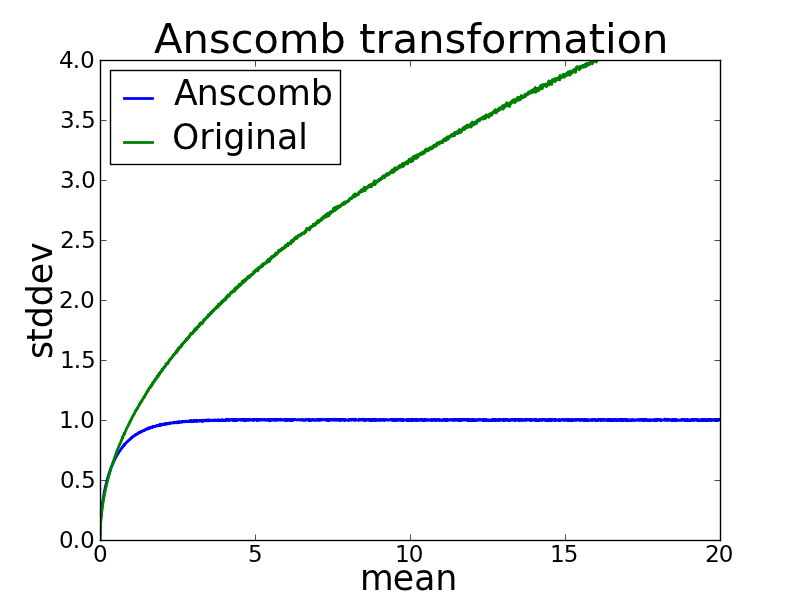
\includegraphics[width = 0.5\textwidth]{pictures/anscombe.png}
	\caption{Standard deviation over mean intensities of different Poisson
	distributions}
	\label{anscombe}
	
\end{figure}

\section{Estimation of camera gain}
The 

\section{Distributions}
\subsection{Poisson distribution}
One very important probability distribution in physics is the Poisson
distribution. It describes the results of ``counting experiments'' and is
therefore very important for image processing as the pictures taken with a
camera are in principle counts of photons reaching the camera. Photon counting
noise is one important example.\\
Poisson distributions are just defined for integer values and the variance is
the same as the mean value of the distribution. Another important attribute is
the skewnes which is the inverse of the squarerot of the mean or variance and describes the assymetry.\\ 
The probability mass function is:
\begin{equation}
	p(n,\mu) = \frac{\mu^n}{n!}\exp(-\mu)
\end{equation}
\subsection{Skellam distribution}
The probability
mass function of a Skellam distribution is a function of the difference between
two Poisson random variables
\begin{equation}
	p(k;\mu_1, \mu_2) =
	\exp(-(\mu_1+\mu_2))\left(\frac{\mu_1}{\mu_2}\right)^{k/2}~I_{|k|}\left(2\sqrt{\mu_1
	\mu_2}\right)
\end{equation}  
where $n_1$, $n_2$ are the Poisson random variables and $k = n_1 - n_2$.
$I_{|k|}$ means the modified Bessel function of the first kind.\\
Mean $\mu$ and variance $\sigma$ of the Skellam distribution are given by
\begin{align}
	&&\mu &= \mu_1 - \mu_2,& \sigma^2 &= \mu_1 + \mu_2\\
	\Rightarrow &&\mu_1& = \frac{\mu + \sigma^2}{2},& \mu_2 &=\frac{-\mu +
	\sigma^2}{2}
\end{align} 

\subsection{Approach using skewness of poisson distribution}
For every pixel there is a set of multiple values in the set. This allows to
calculate the different parameters individually for each pixel. One can
calculate mean and variance of the measured intensities $I_\text{meas}(i,j)$ and
gets
\begin{align}
	\text{mean}(I_\text{meas}(i,j))& = \text{mean}(I_\text{true}(i,j)) + o\\
	\text{var}(I_\text{meas}(i,j))& = g\cdot\text{var}(I_\text{true}(i,j))\\
\end{align}
Assuming a Poisson distribution as the true intensity, mean and variance would
be the same. Unfortunately the mean true intensities are unknown and it is
not possible to determin $g$ and $o$ so far. For large mean Intensities $\mu$
the Poisson distribution becomes more and more similar to a Gauss distribution
with the same mean. However, for small means, the Poisson distribution is not
symmetric. The skewness $s_p$ of a Poission distribution is the inverse of the
square root of the mean $(\mu)^{-.5}$. It can also be directly
calculated from data
\begin{equation}
	s_p = \frac{1}{n}\sum_{i = 1}^n \left(\frac{x_i - \bar x}{\sigma}\right)^3
\end{equation}
The skewness is invariant to shift and multiplication with a constant. This
means that the transformation caused by the camera gain and the dark current
does not affect the skewness. This gives a third equation to solve for $g$ and
$o$.\\
This approach has very strict limitation to at least for background not to
intense signals. If the mean of the true Poisson distributin is higher than
roughly 30 the skewness gives due to noise no stabel results and it is
impossible to determin the mean intensity in this way.
\chapter{ISBI Challenge 2013}
\section{Introduction}
The goal of the ISBI Challenge, as announced on their website (\cite{challenge}), is to give an overview and understanding of availible algorithms for single particle localization microscopy. The focus was on 2d localisation, to give information about the depth of a localisated spot was optional. To benchmark results one needs groundtruth. Therefore the organisers created synthetic datasets of biologically relevant structures such as tubulins. To match realistic conditions the data was transformed to introduce different kinds of noise and background to it.\newline
The participants were given training data sets and the corresponding groundtruth and one month before the deadline of the challenge the test sets. There were two different kind of datasets in principle. One with very dense spots and shorter sequences, the other with longer sequences and fewer spots per frame.\newline
All paricipants were asked to submit their results and also the time it took to run the algorithm and the hardware configuration of the used system.

\section{Terminology}
To be able to compare different algorithms there must be a way to determine the correctly detected spots. To do so for each estimated positon of a flourophor, the nearest correct position of the molecule in the groundtruth data was searched within a lateral tolerance disc. Once a match was found this two spots were taken out of consideration for the matching.\newline
One important parameter for this evaluation is the radius of the lateral tolerance disk, because it has big influence on the number of detections considered to be true positives (TP).\newline
Detections with no associated spot in the groundtruth are called false positives (FP), spots in the groundtruth with no matching detection are called false negatives (FN).\newline
This matching is done frame by frame, it is not possible to match a point from different frames even if the $x$ and $y$ coordinates match perfectly but the frame differs.\newline
The precision ($p$) of a classification task is defined as the ration between the number of true positives and the sum of true positives and false positives:
\begin{equation}
\text{precision: }p = \frac{\text{TP}}{\text{TP}+\text{FP}} 
\end{equation}
It is a number between 0 at worst and 1 at best, telling how reliable the result is, how likely it is that a labeld sample really belongs to the predicted class. In this context it means how certain a detected spot has its origin in a fluorophore attached to the investigated structure and it's origin is not wrongly detected background noise.\newline
An other important value is the recall $r$ that is defined as the ratio of true positives and the sum of true positives and false negatives:
\begin{equation}
\text{recall: }r = \frac{\text{TP}}{\text{TP}+\text{FN}}
\end{equation}
The recall lies also in a range from 0 to 1  and gives an impression on how many relevant spots were found.

\section{Measures} 
For the evaluation three different measures were used. The f-score index $f$, the Jaccard index $J$ and the rot-mean square distance RSME. 
\begin{eqnarray}
	\text{f-score: }f &=\frac{2\cdot p \cdot r}{p+r} 
\end{eqnarray}
\subsection{Jaccard index}
Let $A$ be the set of points of the groundtruth and $B$ be the set of detected points. The Jaccard index $J$ is defined as:
\begin{equation}
\text{Jaccard: }J = \frac{\left|A\cap B\right|}{\left|A\cup B\right|}
\end{equation}
The intersection is done frame by frame. This means two spots from the groundtruth and the detection set just match if they occure in the same frame. 
\subsection{RSME}
The root-mean square distance gives an impression how big the squared distance between a spot in the groundtruth and an associated detection was in average. It can be calculated like this:
\begin{equation}
\text{RSME} = \frac{1}{\left|A\cap B\right|}\sum\limits_{i=1}^{\left|A\cap B\right|} \left(p_a(x,y)-p_b(x,y)\right)^2
\end{equation}
\section{Trainingsdata}
\subsection{Bundled tubes datasets}
There was two kinds of bundled tubes data sets, both created from the same underlying structure, one set with a high spot density and a short sequence of 360 frames, the other with fewer spots per frame but 12000 frames in total. Picture \ref{bundledtubesHighowDensityFrame} shows one frame of each data set.\newline
\begin{figure}
\begin{minipage}[t]{0.60\textwidth}
\subfloat[High spot density]{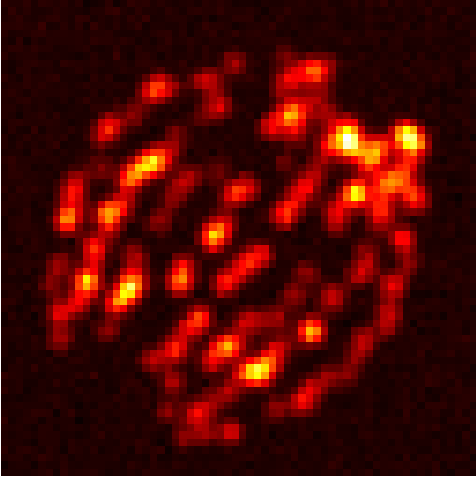
\includegraphics[width = 0.485\textwidth]{pictures/bundledTubesHighDensityFrameFarbig.png}}\hfill
\subfloat[Low spot density]{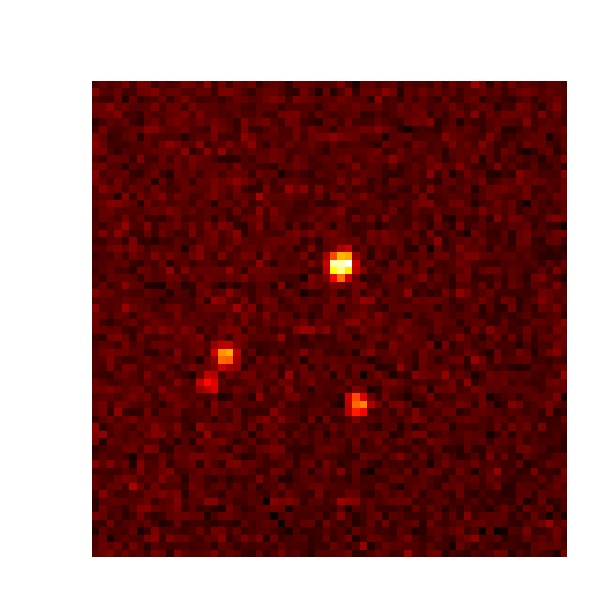
\includegraphics[width = 0.485\textwidth]{pictures/bundledTubesLowDensityFrameFarbig.png}}
	\caption{One frame from bundled tubes training data set}
	\label{bundledtubesHighowDensityFrame}	
\end{minipage}\hfill
\begin{minipage}[t]{0.33\textwidth}
\centering
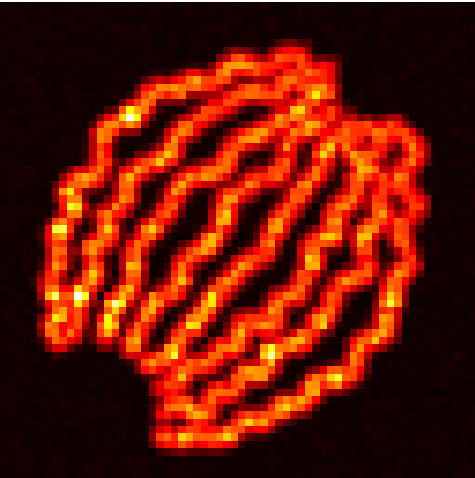
\includegraphics[width = 0.88\textwidth]{pictures/maximumProjectionBundledTubesLSFarbig.png}
	\caption{Maximum projection of bundled tubes data set}
	\label{pctMaximumProjBundledTubes}

\end{minipage}
\end{figure}
The original images very small, just 64 pixels in each dimension. Both sequences had spatial and temporal constant background. Picture \ref{pctMaximumProjBundledTubes} shows the maximum projection of the bundled tubes data set. The maximum projection is used to reduce the dimensionality of a data set. In this case for each pixel in $x$- and $y$-dimension, in the three dimensional dataset, the brightes value from all frames is taken. 


\subsection{Tubulin data sets}
The other training data sets models 7 microtubules, a structure that is a long filament up several micrometers long and a diameter of about 25 nanometers. The spot density lies somewhere between the high density and the low density of the bundled tubes data sets. This data sets show strong inhomogeneity in spatial dimensions and moderate inhomogeneity in temporal dimension, see figure \ref{tubulinVariableBg}. This is the reason why in the lower left corner of the maximum projection \ref{pctMaximumProjTubulin} a brighter area can be seen.

\begin{figure}
\subfloat[Tubulin2 frame 10]{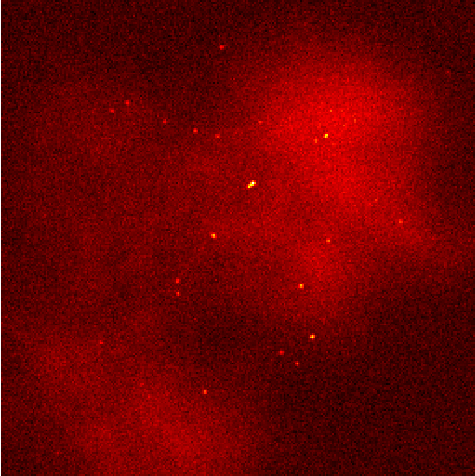
\includegraphics[width = 0.485\textwidth]{pictures/Tubulin2Frame10.png}}\hfill
\subfloat[Tubulin2 frame 1010]{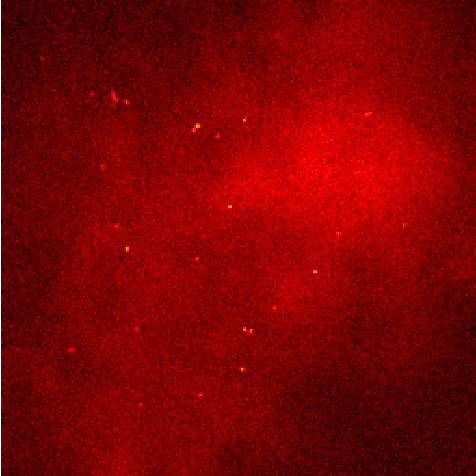
\includegraphics[width = 0.485\textwidth]{pictures/Tubulin2Frame1010.png}}
	\caption{This pictures show the variability of the background in the spatial and temporal dimensions}
	\label{tubulinVariableBg}	
\end{figure}

\begin{figure}
\centering
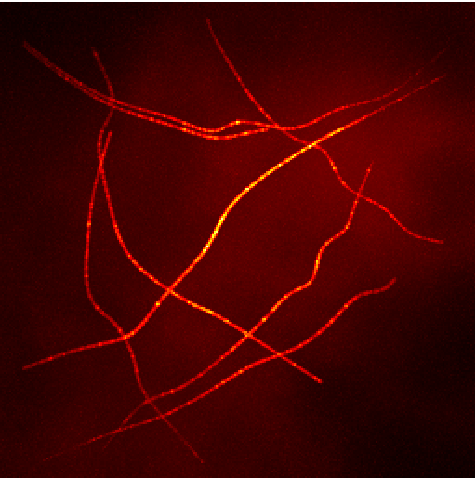
\includegraphics[width = 0.88\textwidth]{pictures/maximumProjectionTubulinFarbig.png}
	\caption{Maximum projection of tubulin data set}
	\label{pctMaximumProjTubulin}


\end{figure}

\section{Submissions}
\subsection{High precision}
\subsection{High score}
\subsection{Highest score via postprocessing}
\section{Results}
\chapter{Check of the assumptions}
The whole workflow depends on some assumptions about the data or the results of certain transformations. This assumptions have to be met at least roughly to ensure the correctness of the results.\newline
This section gives proofs for most of the assumptions like accuracy of the PSF scale estimation or that the matched filter of the matching size compared to the PSF performs best.
\section{Calibration measurement}
As described by \cite{meanVar} the gain can be determined using the mean and variance using data with different mean intensities. Therefore a calibration dataset was aquired. The temperature and the gain factor were set to be like the settings usuall used. A sample with cells was prepared for the Storm measurement. First eleven time series were taken, with opend shutter and with increasing exposure time from 0 milliseconds up to 1000 milliseconds. Afterwards the same procedure were repeated with the shutter kept closed. Figure \ref{calibplot} shows the results for the first 6 exposure time. All the points lie on a straight line. The gain factor determined from the calibration measurement was 3.9, the offset 315. This offset is too small. An other methode was used to determine the offset. There were also an other series of  images taken with closed shutter. This series shows the response of the camera without any light around. The mean value of the shortest exposure time were taken as offset. The value is 380. 
\begin{figure}
\centering
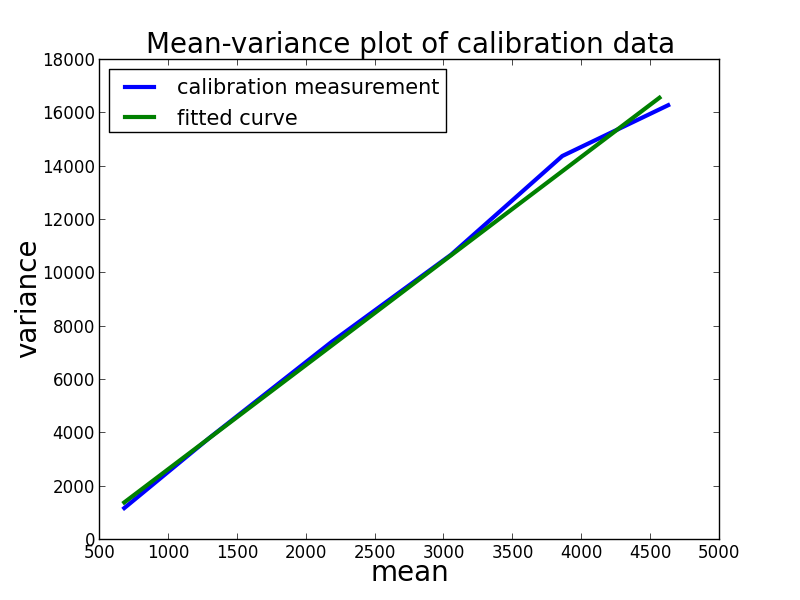
\includegraphics[width = 0.88\textwidth]{pictures/meanVariancePlotCalibration.png}
	 \caption{Result of the calibration measurements. The gain determined from this variance-mean plot is 3.9.}
	\label{calibplot}
\end{figure}


\section{Correction to Poisson distributions}
It is very important for the whole workflow that the first transform results in background intensities that follow a Poisson distribution. To test this a real world image was transformed with parameters taken from the calibration measurement described in the previous section. The offset was estimated from the minimal intensity of the raw image. The histograms for two generic background pixels are shown in figure \ref{isitPoisson}. A Poisson distribution with the mean of the pixels intensities is also shown in the figures. This histograms were aquired using the pixel intensities of one pixel for 3000 frames. The histogram matches the expected Poisson distribution.
\begin{figure}
\subfloat[Tubulin2 frame 10]{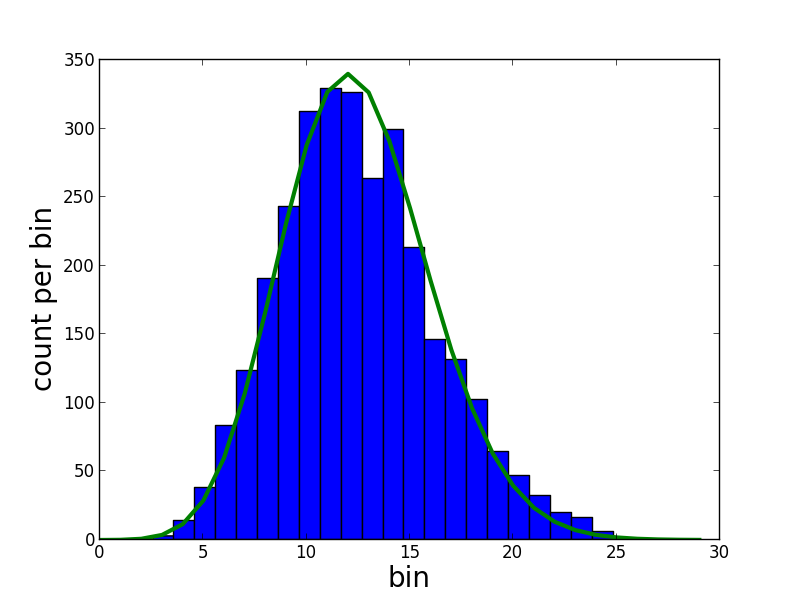
\includegraphics[width = 0.485\textwidth]{pictures/IsItPoisson105_105.png}}\hfill
\subfloat[Tubulin2 frame 1010]{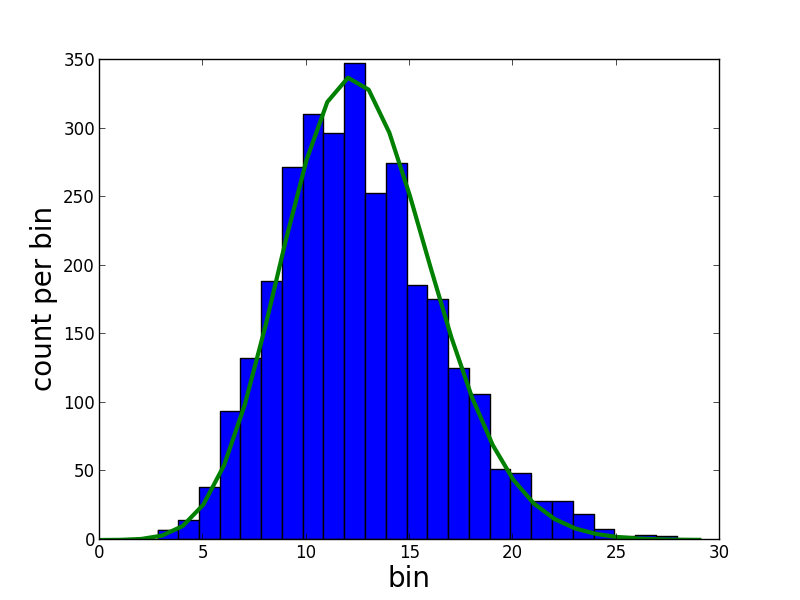
\includegraphics[width = 0.485\textwidth]{pictures/IsItPoisson50_50.png}}
	\caption{This pictures show how well the histograms of background pixels taken over the first 3000 frames, follow a Poisson distribution. For the gain the parameter from the calibration measurement of $g$ = 3.9 were used. The offset was estimated from the minimal intensities of the original image.}
	\label{isitPoisson}	
\end{figure}

\section{Result Anscombe transformation}
The same data set used in the previous section was used. After the transformation described in \ref{trafoPoiss}, the Anscombe transformation was aplied and the background subtracted. Figure \ref{isitAnscombe} shows the histogram of the intensities of one randomly chosen frame and a Gaussian with zero mean and unit variance. The histogram fits very well to the Gaussian. The tail exceeding the Gaussian on the right side can at least partially explained by the signal that is present in the image and does not follow the Gaussian distribution, but has higher intensities.
\begin{figure}
\centering
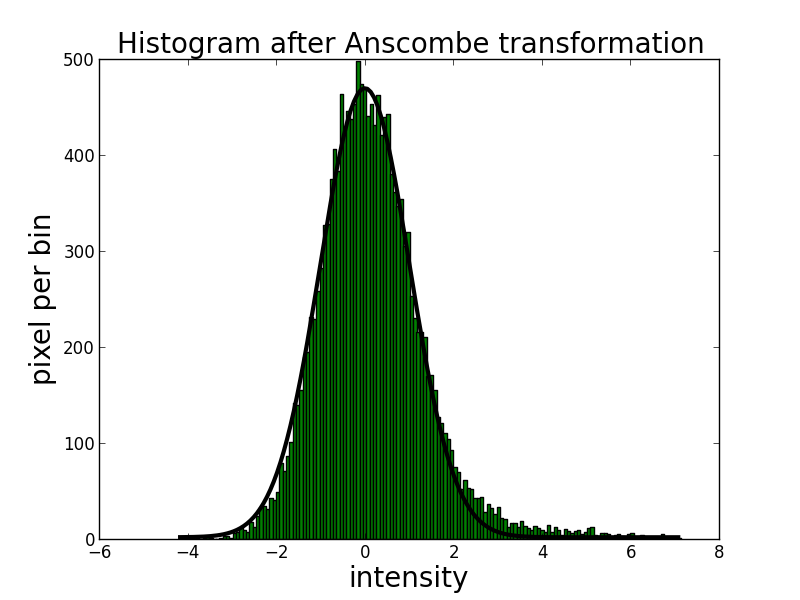
\includegraphics[width = 0.88\textwidth]{pictures/anscombeAndFit.png}
	 \caption{After the Anscombe transformation the background pixel intensities should be distributed with mean zero and variance one. This figure shows the histogram of the pixel intensities and a fitted gaussian with variance one and mean zero.}
	\label{isitAnscombe}
\end{figure}

\section{Accuracy of detection}
Unfortunately the position of the flourescent molecules can't be detected
perfectly. There are three main contribution to the error in detection.\\
On the one hand, there is the problem of finding the maximum in a noisy signal. Due to
noise the pixel next to the true maximum might gain some intensity and be
therefore brighter.\newline
On the other hand, the position is deteted by upscaling the pixel grid and interpolation.
After that the maximums position of the upscaled grid is taken as the resulting
position. This gives an error from roughly a 12th pixelwidth. This error becomes less important with higher upscaling factors.\newline

Because there is no groundtruth for the real data, one has to produce test data and groundtruth. This was done simular to the method described by \cite{simulated}. The difference was, that instead of generating just one spot per frame a different number of spots were simulated for each frame. For different signal to  noise ratios, a dataset with 40 times 40 pixels and 1000 frames was created. Each frame containing one, three or five point spread functions. The position of the spots was determined beforehand, to use the same spots for each signal to noise ratio.\newline

To determine the accuracy the standard deviation between the true position of the signal and its detection were used. For data sets with more than one spot per frame, it was searched for the best match within a certain distance around the true position. If a pair of true spot and detection was found, both were removed for further matching of the remaining signals. In the end the averaged standard deviation of the detection relative to the true positions were calculated as follows:
\begin{align}
	\text{std. dev.} = \sum_i \sqrt{\left(\bf{p}_{\text{true}}^i - \bf{p}_{\text{detec}}^i\right)^2}
\end{align}
$i$ runs over all found pairs of groundtruth and detections, $\bf{p}$ describes the two dimensional spatial vector of the groundtruth or detection respectivly.\newline

The results can be seen in \ref{accplot}. It can be seen, that the more spots are present per frame the harder it is to detect them properly. This is a result of the fact that spots that lay near each other might be detected as just one spot, what gives rise to higher errors in the detection accuracy.


\begin{figure}
\begin{minipage}[t]{0.48\textwidth}
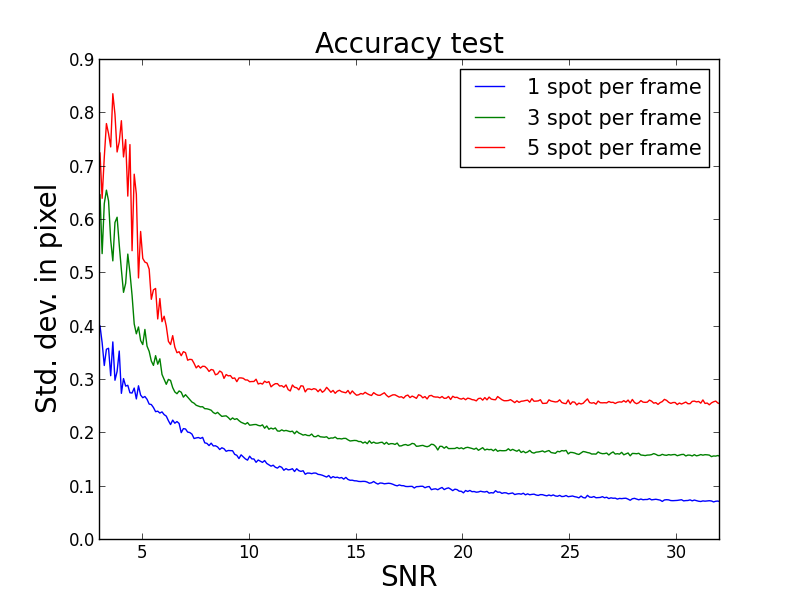
\includegraphics[width = 0.99\textwidth]{pictures/AccuracyTest.png}
	\caption{Result of the accuracy test. For datasets with one, three or five point spread functions per frame, evaluated for different signal to noise levels. The more dense the spots are the less accurate the detections are.}
	\label{accplot}	
\end{minipage}\hfill
\begin{minipage}[t]{0.48\textwidth}
\centering
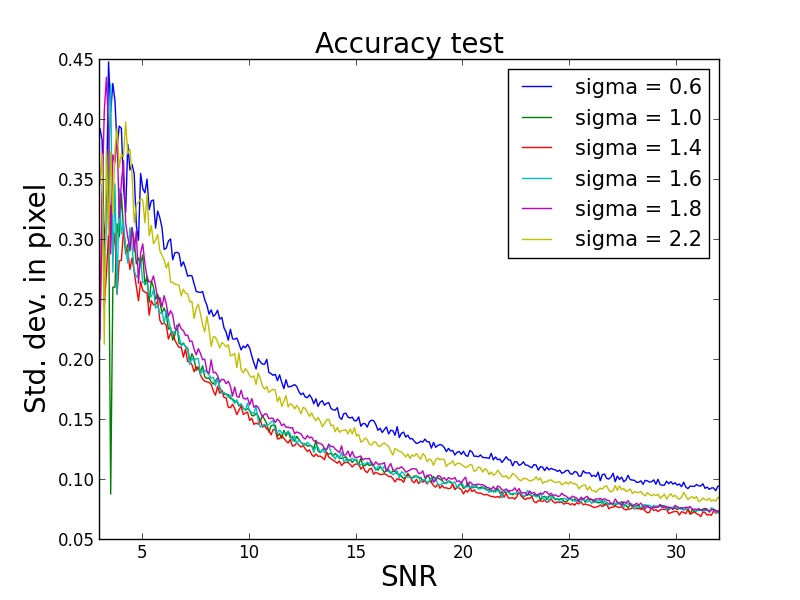
\includegraphics[width = 0.99\textwidth]{pictures/AccuracyTestSigma.png}
	\caption{Result of the accuracy test for different sigmas for the gaussian smoothing. One data set was processed with different sigma values and evaluated for different signal to noise levels. The true standard deviation of point spread function of the simulated data is 1.4.}
	\label{accplot2}

\end{minipage}
\end{figure}


\section{Matched filter is best filter} \label{detectionError}
For denoising the image a matched filter is used. Since we assume the point spread function to be gaussian, a two dimensional gaussian filter with the estimated size of the point spread function is used. The following calculation shows why this is the best choice for the standard deviation.\newline
This calculation is similar to the calculation in \cite{ulli}. The assumptions are, the point spread function is gaussian shaped with a true standard deviation of $\sigma_\text{PSF}$, the image contains white gaussian noise with mean zero and unit variance, the applied filter for denoising is a gaussian filter with standard deviation $\sigma_\text{filter}$.\newline
The image $f$ is composed of gaussian filter convolved with the signal $s$ and the above mentioned white noise $n$. $s$ and $n$ are describing the filtered signal respectivly noise.
\begin{align}
 f=s+n \label{gl91}
\end{align}
Without noise the first derivative of $f$ which is equal to $s$ in the noise-free case vanishs at the center of the gaussian signal. This center can be set to the origin without losing generality. But noise shifts the zero crossing of the first derivatives to $\Delta x,~\Delta y$. For now just one dimension is considered.
\begin{align}
\frac{\partial f}{\partial x}\left(\Delta x, \Delta y\right) &= \frac{\partial s}{\partial x} \left(\Delta x, \Delta y\right) + \frac{\partial n}{\partial x}\left(\Delta x, \Delta y\right)&=0
\end{align}  

Using Taylor expansion around $x = 0$ at $y= 0$ for the signal, yields:
\begin{align}
f_x(\Delta x, \Delta y)&\approx \underbrace{s_x(0, 0)}_{=0} + s_{xx}(0, 0)\cdot \Delta x + n_x(\Delta x, \Delta y)&=0\\
\Rightarrow \text{var}(s_{xx}(0, 0)\cdot \Delta x)&= \text{var}(n_x(\Delta x,\Delta y)\\
\Rightarrow \text{var}(\Delta x) &= \frac{\text{var}(n_x(\Delta x, \Delta y)}{s_{xx}^2(0, 0)} \label{ch9gl1}
\end{align}

The result for the variance of the first derivative of white noise convolved with a gaussian filter of width $\sigma_\text{filter}$ can be found at \cite{ulli}. It is:
\begin{align}
	\text{var}(n_x) = \frac{N^2}{8\pi\sigma_\text{filter}^4},~\text{with }N\text{: noise std. dev} \label{ch9gl2}
\end{align}
The convolution of the Gaussian PSF  with an other Gaussian results in Gaussian with combined scales.
\begin{align}
 \mathcal{N}(0,\sigma_\text{PSF}) \ast \mathcal{N}(0,\sigma_\text{filter}) = \mathcal{N}\left(0,\underbrace{\sqrt{\sigma_\text{PSF}^2+\sigma_\text{filter}^2}}_{=\sigma_\text{comb}}\right)
\end{align}
The value of the second derivative in $x$-direction of the convolved PSF at (0,0) is:
\begin{align}
 \frac{\partial^2 S_0\cdot\mathcal{N}\left((\mu_x,\mu_y),\sigma_\text{comb}\right)}{\partial x^2}  &=  -\frac{S_0}{2\pi \sigma_\text{comb}^4}  \label{ch9gl3}
\end{align}
Combining \ref{ch9gl1}, \ref{ch9gl2} and \ref{ch9gl3} yields:
\begin{align}
\text{var}\left(\Delta x\right) &= \dfrac{\dfrac{N^2}{8\pi\sigma_\text{filter}^4}}{\dfrac{S_0^2}{4\pi^2 \sigma_\text{comb}^8}}\\
&= \frac{N^2\cdot 4\pi^2 \sigma_\text{comb}^8}{S_0^2\cdot8\pi\sigma_\text{filter}^4}\\
&= \frac{N^2}{S_0^2} \frac{\pi \left(\sigma_\text{filter}^2+\sigma_\text{PSF}^2\right)^4}{2\sigma_\text{filter}^4}\\
&= \frac{N^2\pi}{2S_0^2} \left(1+\frac{\sigma_\text{PSF}^2}{\sigma_\text{filter}^2}\right)^2\left(\sigma_\text{filter}^2+\sigma_\text{PSF}^2\right)^2 
\end{align}
The same variance can be calculated with respect to $y$, yielding a total variance that is square root of 2 bigger, because the variances are orthogonal.
Therefore the standard deviation of the localisation is:
\begin{align}
 \text{std. dev loc}&=\frac{N}{S_0}\sqrt{\frac{\sqrt{2}\pi}{2}}
 \left(1+\frac{\sigma_\text{PSF}^2}{\sigma_\text{filter}^2}\right)\left(\sigma_\text{filter}^2+\sigma_\text{PSF}^2\right) 
\end{align}
To verify this results a test data sets has been created containing 3500 frames with one PSF with different scales. This data sets have been filtered with Gaussian filters of different sizes. After that the maximum for each frame was detected and compared with the true position. Figure \ref{matchedFilter1} shows the accuracy for different PSF scales and filter widths.\newline
As expected the best results were achieved using a Gaussian filter with the PSFs size. The larger the PSFs scale the more inaccurate the localisation becomes.\newline

\begin{figure}
\centering
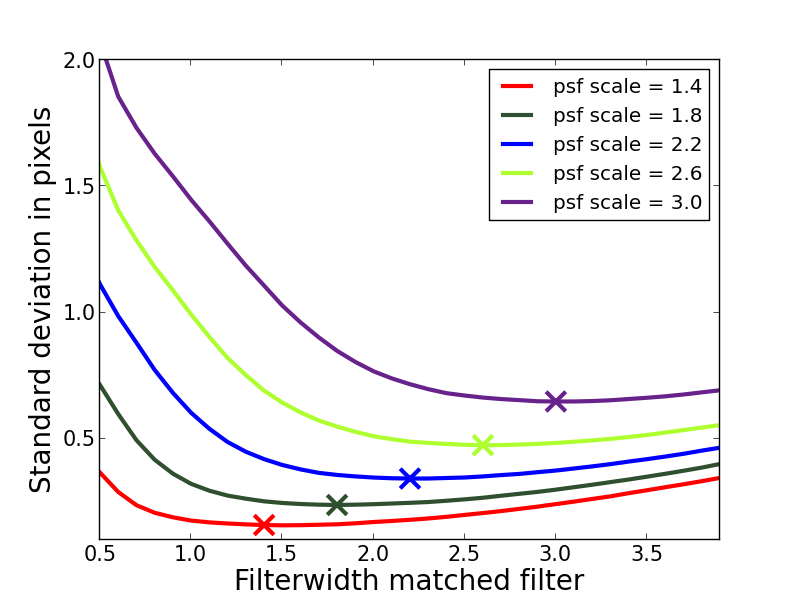
\includegraphics[width = 0.88\textwidth]{pictures/matchedFilterPlots1.png}
	 \caption{This figure shows the accuracy of detection achieved using different Gaussian filters for denoising. The cross marks the minima of the curves.}
	\label{matchedFilter1}
\end{figure}

The figures in \ref{matchedFilter2} show the measurement, a shifted measurement curve and the result of the calculation. The measured error was larger than the calculated error, therefore the shifted line is also shown to state that the curves shape match but there is an additional error that shifts the line. \newline
This results show that the calculated standard deviation of the localisation can be used to estimate the localisation error of SimpleSTORM for further calculations or error propagation.

\begin{figure}
\subfloat[PSFs scale = 2.6]{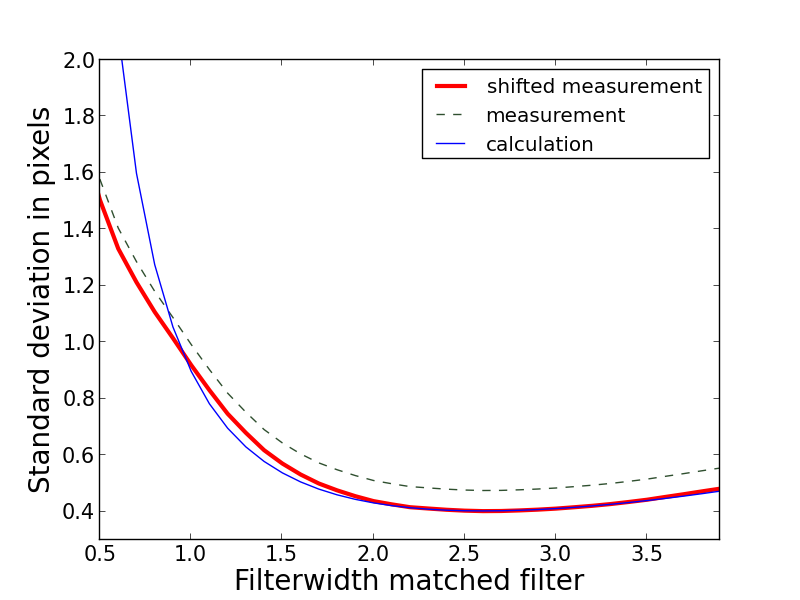
\includegraphics[width = 0.485\textwidth]{pictures/matchedFilterPlots2.png}}\hfill
\subfloat[PSFs scale = 1.8]{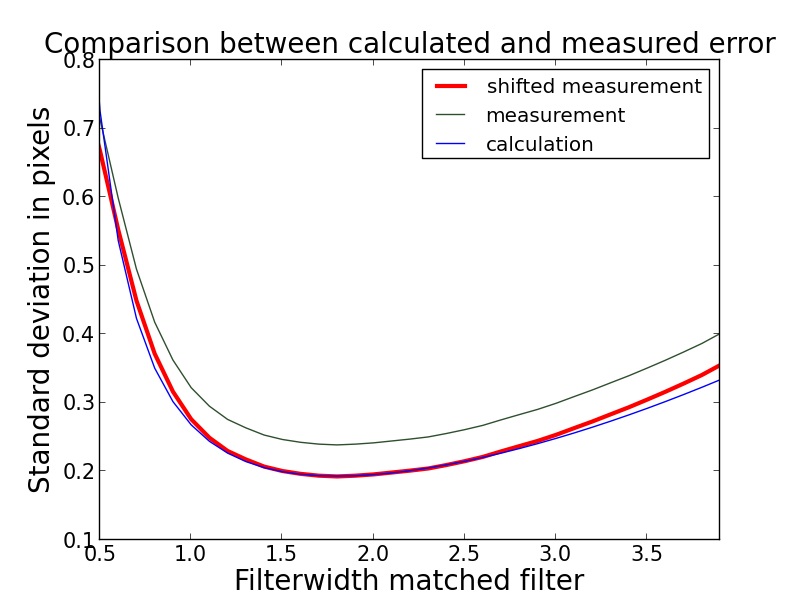
\includegraphics[width = 0.485\textwidth]{pictures/matchedFilterPlots3.png}}
	\caption{Comparison between the measured and the calculated localisation error. The dashed lines show the unchanged measurements results, for better comparism the line was shifted to match the calculated error.}
	\label{matchedFilter2}	
\end{figure}

\section{Test PSF estimation}
The estimation of the width of the point spread function of the signal is very important. The localisation error increases with larger deviations of the matched filters width from the true width of the PSF. Figure \ref{estimatedSigma} shows the results of an accuracy test. For this test data was created artificially. One PSF was simulated at a random location with a fixed width, poisson noise was added so that the signal-to-noise ratio was 10. Then this width was estimated by the SimpleSTORM algorithm. This was done with values for the standard deviation of the gaussian in a range from 0.2 up to 4. The plot shows that for standard deviations up to 2.5 the estimated value for the width is very close to the actual value. The wider the PSF becomes in the spatial domain the smaller it gets in the Fourier domain. This is the reason why the accuracy of the estimation is decreasing for larger widths. This effect can be reduced by choosing a larger region of interest for the power spectrums acumulation. The parameter chosen for the plot in figure \ref{estimatedSigma} was the default value. The typical width of the PSF is in a range of 1 to 2, this is a range in which the estimation gives reliable results.\newline
\begin{figure}
\centering
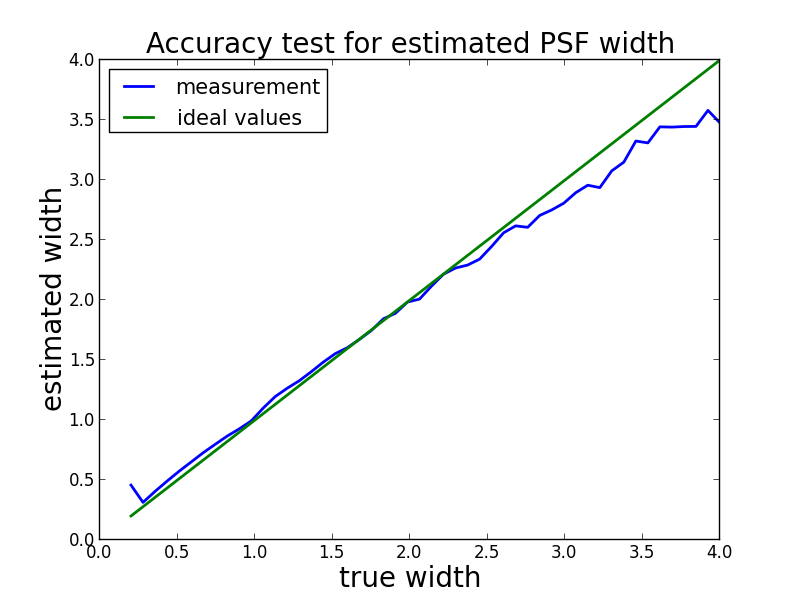
\includegraphics[width = 0.88\textwidth]{pictures/AccuracyTestPSFWidth.png}
	 \caption{The figure shows the estimated widths of the point spread function plotted over the true widht of the simulated signal. The signal-to-noise ratio was 10 for this test. The green line shows the correct results.}
	\label{estimatedSigma}
\end{figure}


\section{Bleaching signal}
One assumption was that the backgrounds illumination is caused mainly form out of focus fluorophors and therefore Poission distributed. If this is the case the background illumination should decrease over time. Bleaching of flourophores describes the process in which the flourescent molecules change their conformation and lose the ability to emit light or the spectrum of the emission changes so that they can't be detected any more. All flourophores used for the STORM images we got are bleaching over time. This decay of the mean backgrounds intensity is shown in figure \ref{bleaching}.

\begin{figure}
\centering
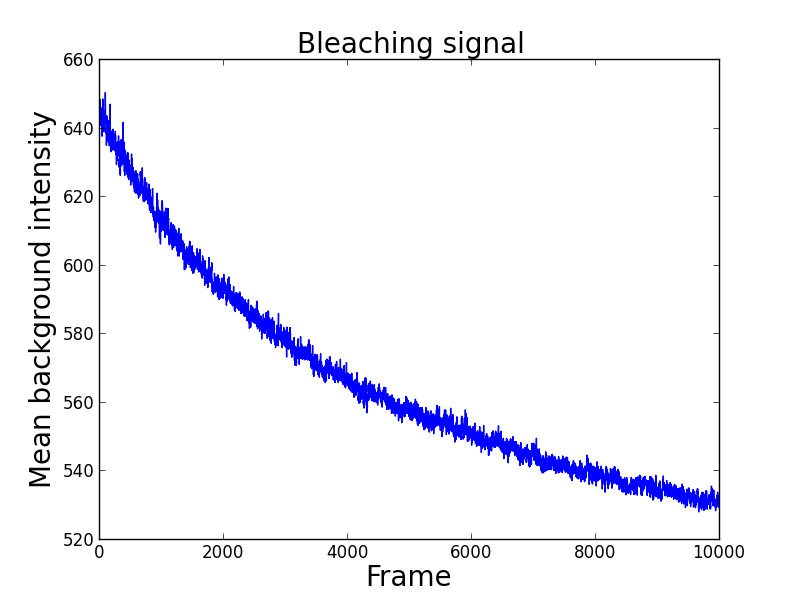
\includegraphics[width = 0.5\textwidth]{pictures/bleaching.png}
	\caption{The number of active fluorophores decrease over time and so does the mean intensity of the image. This picture shows the mean intensities over 10 background pixel over time. }
	\label{bleaching}
\end{figure}

\chapter{Appendix}


\listoffigures
\listoftables

\section{Additional tables of ISBI challenge results}

%\begin{table}[H]
\begin{center}
%\caption{Results for the main submission (with postprocessing)}
\begin{minipage}{\textwidth}
\captionof{table}{Results for the main submission for the high density data set (with postprocessing)}\label{reshd1}%
\begin{tabular}{lrrrr}
Dataset&Jaccard (in \%)&Precsision (in \%)& Recall (in \%) & RMSE (in nm)\\
HD1&40.44&100&41&40.13\\
HD2&30.84&100&31&63.18\\
HD3&12.55&100&13&61.8
\end{tabular} 
\end{minipage}
\end{center}
%\end{table}


%\begin{table}[H]
\begin{center}
\begin{minipage}{\textwidth}
\captionof{table}{Results for the high precission submission for the high density data set}\label{reshd2}
\begin{tabular}{lrrrr}
Dataset&Jaccard (in \%)&Precsision (in \%)& Recall (in \%) & RMSE (in nm)\\
HD1&37.62&100&38&40.23\\
HD2&28.37&100&28&60.70\\
HD3&12.66&100&13&62.58
\end{tabular}
\end{minipage}
\end{center}
%\end{table}

\begin{center}
\begin{minipage}{\textwidth}
\captionof{table}{Results for the high score submission for the high density data set (without postprocessing)}\label{reshd3}
\begin{tabular}{lrrrr}
Dataset&Jaccard (in \%)&Precsision (in \%)& Recall (in \%) & RMSE (in nm)\\
HD1&37.96&100&38&40.22\\
HD2&29.73&94&30&63.33\\
HD3&13.00&99&13&63.95
\end{tabular}
\end{minipage}
\end{center}


\begin{center}
\begin{minipage}{\textwidth}
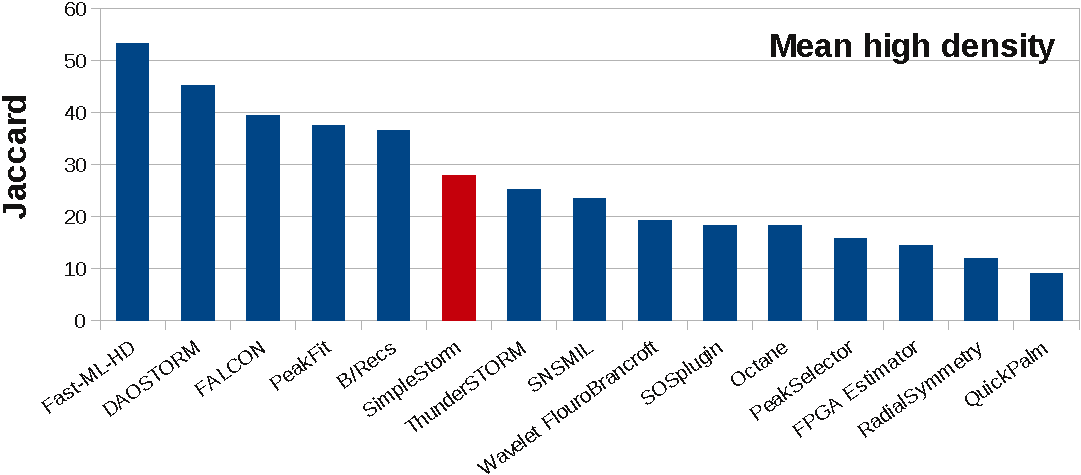
\includegraphics[width = 0.88\textwidth]{pictures/diagrammsChallenge/MeanHighDensityJaccardCropped.pdf}
	\captionof{figure}{Results for high density data sets. The Jaccard indices are averaged over all three data sets. For this score higher is better.}
	\label{meanJaccardHighDensity}
	\end{minipage}
\end{center}

\begin{center}
\begin{minipage}{\textwidth}
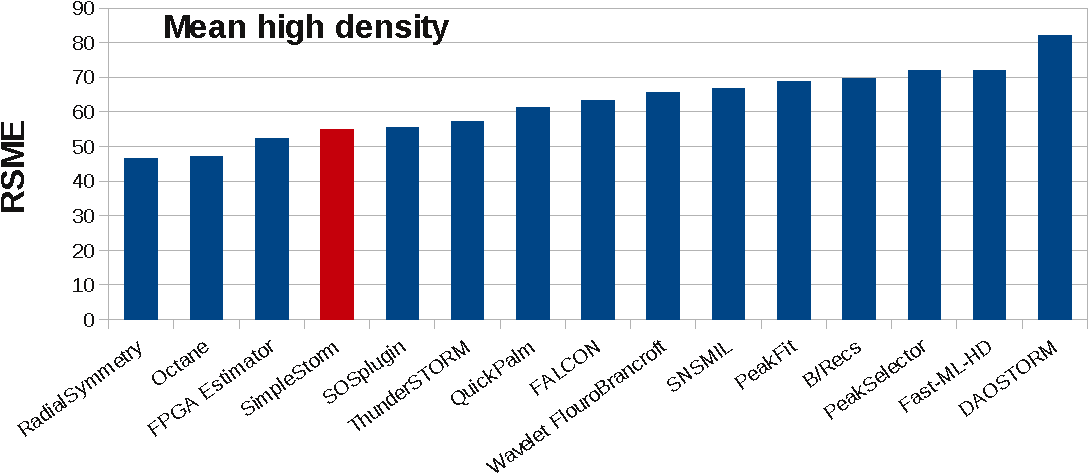
\includegraphics[width = 0.88\textwidth]{pictures/diagrammsChallenge/MeanHighDensityRSMECropped.pdf}
	\captionof{figure}{Results for high density data sets. Averaged RSME scores over all three datasets. For this score lower is better.}
	\label{meanRSMEHighDensity}
	\end{minipage}
\end{center}



\begin{center}
\begin{minipage}{\textwidth}
\captionof{table}{Results for the main submission for low density data sets(with postprocessing)}
\begin{tabular}{lrrrr}
Dataset&Jaccard (in \%)&Precsision (in \%)& Recall (in \%) & RMSE (in nm)\\
LS1&86.12&100&86&26.32\\
LS2&69.64&97&71&37.43\\
LS3&47.48&99&48&54.2
\end{tabular}\label{resls1}
\end{minipage}
\end{center}


\begin{center}
\begin{minipage}{\textwidth}
\captionof{table}{Results for the high precission submission for low density data sets}\label{resls2}
\begin{tabular}{lrrrr}
Dataset&Jaccard (in \%)&Precsision (in \%)& Recall (in \%) & RMSE (in nm)\\
LS1&83.39&100&83&27.91\\
LS2&63.21&100&63&39.57\\
LS3&40.82&100&41&49.55
\end{tabular}
\end{minipage}
\end{center}

\begin{center}
\begin{minipage}{\textwidth}
\captionof{table}{Results for the high score submission for low density data sets (without postprocessing)}\label{resls3}
\begin{tabular}{lrrrr}
Dataset&Jaccard (in \%)&Precsision (in \%)& Recall (in \%) & RMSE (in nm)\\
LS1&87.23&99&88&28.10\\
LS2&65.95&89&72&44.60\\
LS3&40.82&96&48&54.40
\end{tabular}
\end{minipage}
\end{center}



\begin{center}
\begin{minipage}{\textwidth}
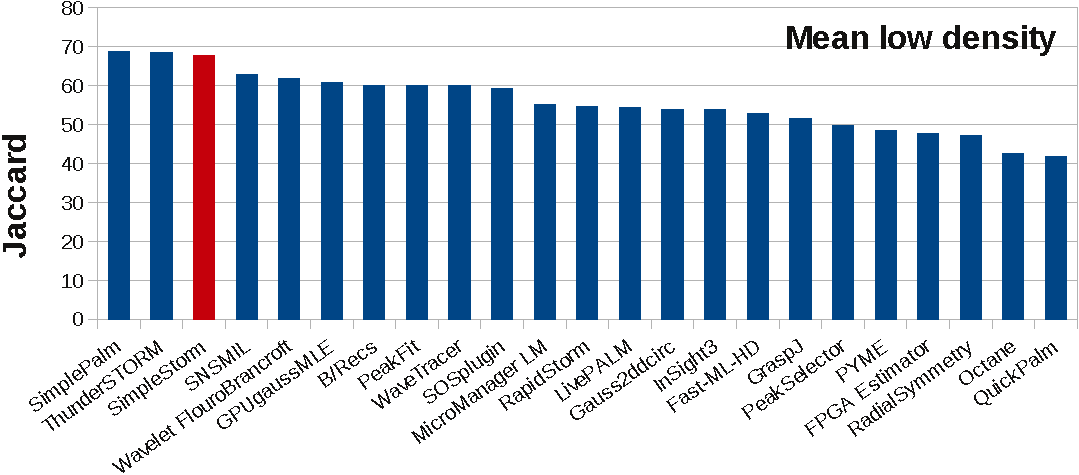
\includegraphics[width = 0.88\textwidth]{pictures/diagrammsChallenge/MeanLowDensityJaccardCropped.pdf}
	\captionof{figure}{Results for low density data sets. The Jaccard indices are averaged over all three data sets. For this score higher is better.}
	\label{meanJaccardLowDensity}
\end{minipage}
\end{center}

\begin{center}
\begin{minipage}{\textwidth}
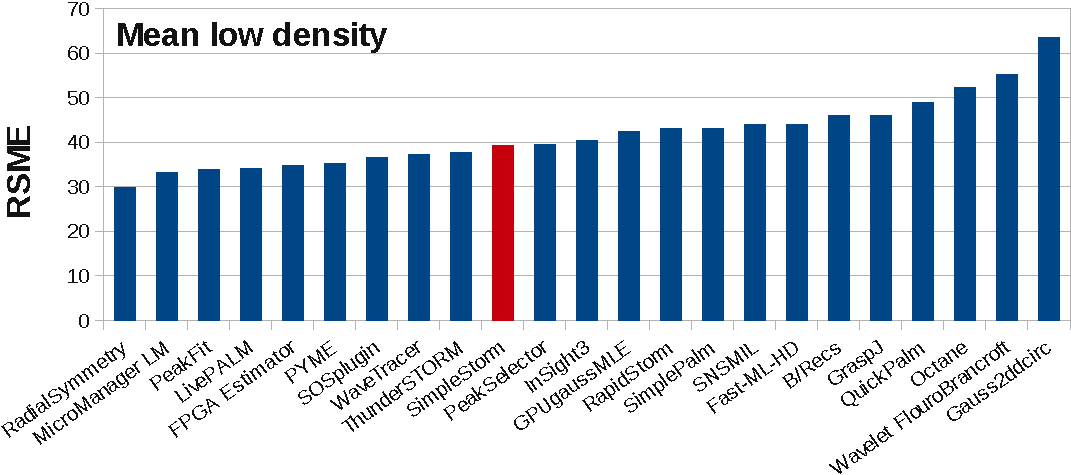
\includegraphics[width = 0.88\textwidth]{pictures/diagrammsChallenge/MeanLowDensityRSMECropped.pdf}
	\captionof{figure}{Results for low density data sets. Averaged RSME scores over all three datasets. For this score lower is better.}
	\label{meanRSMELowDensity}
\end{minipage}
\end{center}

\begin{center}
\begin{minipage}{\textwidth}
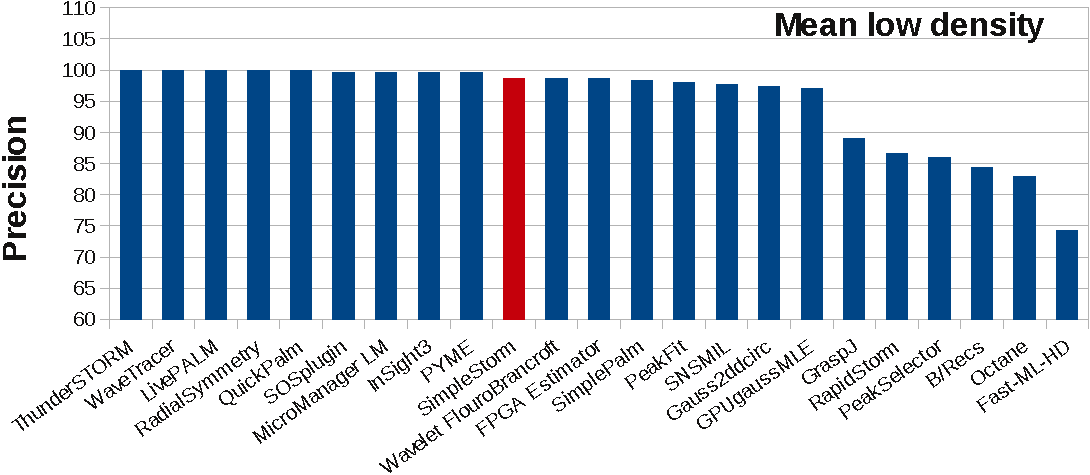
\includegraphics[width = 0.88\textwidth]{pictures/diagrammsChallenge/MeanLowDensityPrecisionCropped.pdf}
	\captionof{figure}{Results for low density data sets. Averaged Precision over all three datasets. For this score higher is better. The y axis is broken to show the differences better.}
	\label{meanPrecisionLowDensity}
\end{minipage}
\end{center}

\begin{center}
\begin{minipage}{\textwidth}
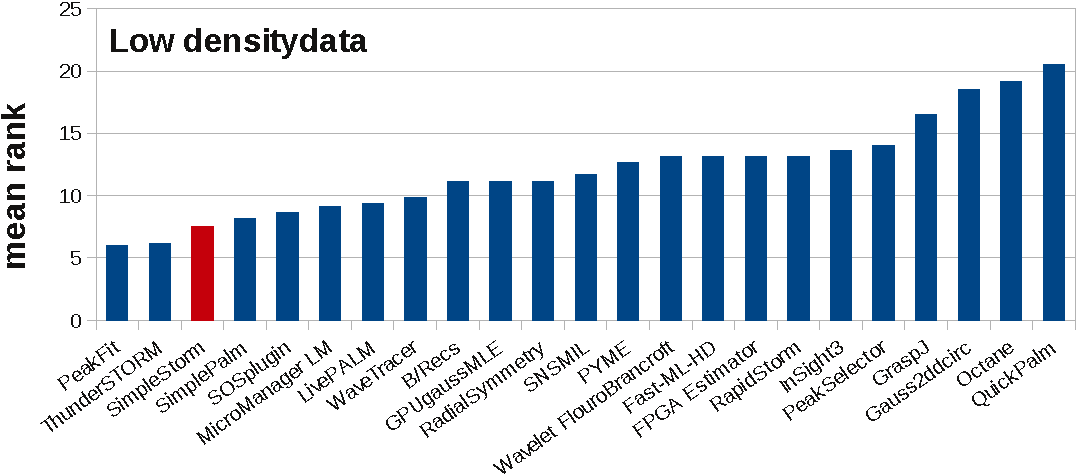
\includegraphics[width = 0.88\textwidth]{pictures/diagrammsChallenge/MeanRankLowDensityCropped.pdf}
	\captionof{figure}{Averaged rank over Jaccard index and RSME score for all low density data sets. Lower ranks are better.}
	\label{meanRankLow}
\end{minipage}
\end{center}

\begin{center}
\begin{minipage}{\textwidth}
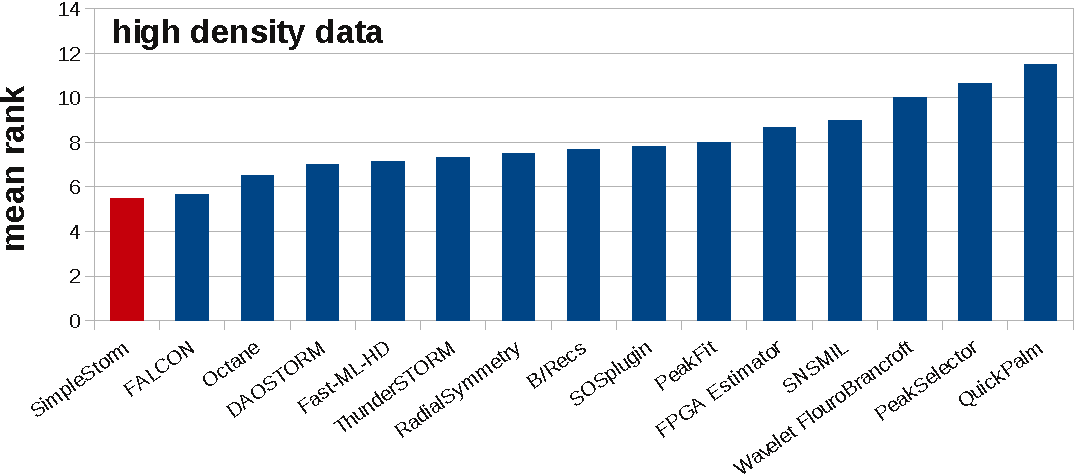
\includegraphics[width = 0.88\textwidth]{pictures/diagrammsChallenge/MeanRankHighDensityCropped.pdf}
	\captionof{figure}{Averaged rank over Jaccard index and RSME score for all high density data sets. Lower ranks are better}
	\label{meanRankHigh}
	\end{minipage}
\end{center}
%\newpage
Erkl\"arung:
\\
\\
\\
\\
Hiermit versichere ich, dass ich diese Master Arbeit selbstst\"andig verfasst habe und keine anderen als die angegebenen Quellen und Hilfsmittel verwendet habe.\\
\\
\\
\\
\\
\\
\\
Heidelberg, den 11. Juni 2013            ....................................

\bibliographystyle{te}

\bibliography{research}

\end{document}
